\documentclass[11pt]{article}
\usepackage[a4paper, total={6in, 8in}]{geometry}
\usepackage{graphicx}
\usepackage{multicol}
\usepackage{multirow}
\usepackage{xcolor}

\title{July2023 CSE300 Week10 Online Evaluation}
\author{Md. Emamul Haque Pranta}
\date{\today}

\begin{document}
    \maketitle
    \tableofcontents

\newpage
\section{RISC Architecture}
\begin{figure}[h]
    \centering
    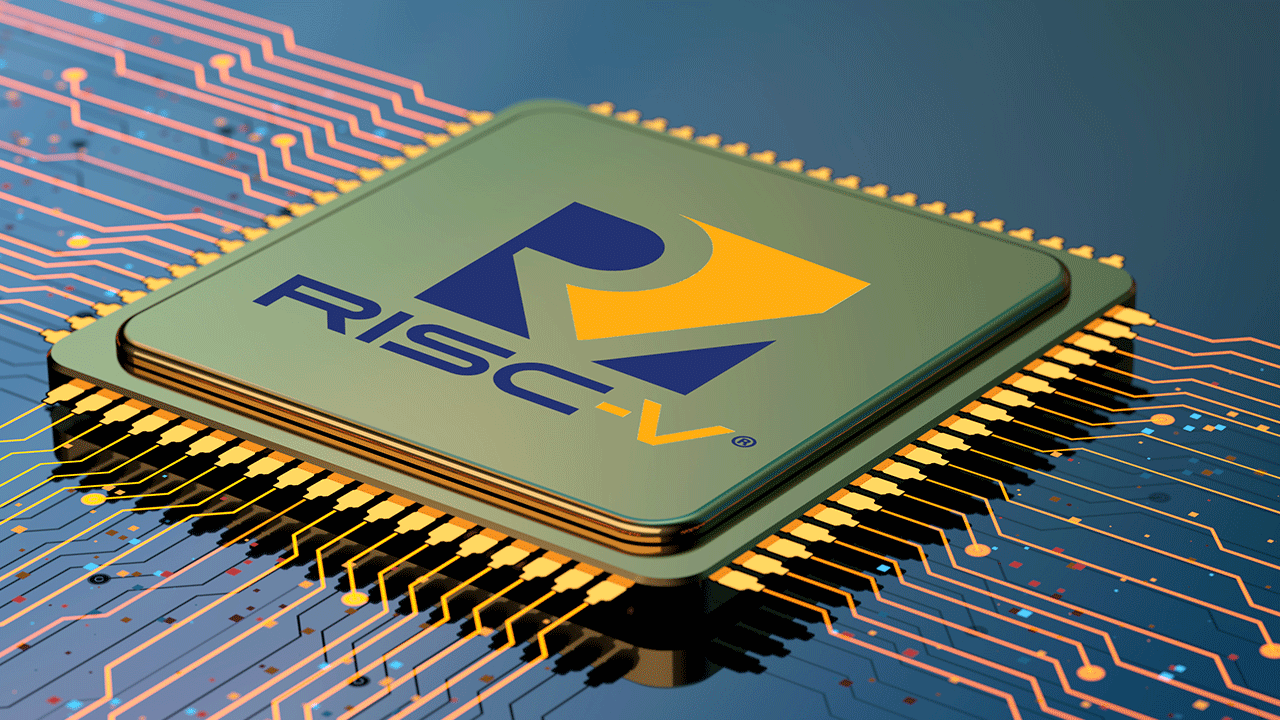
\includegraphics[width=0.9\textwidth]{Images/risc.png}
    \caption{RISC Architecture}
    \label{fig:risc}
\end{figure}

\section{Table in \LaTeX}
\begin{table}[h]
    \centering
    \begin{tabular}{|c|c|c|c|}
        \hline
        \multirow{10}{*}{numeric literals} & \multirow{5}{*}{integers} & in decimal & 8743 \\
        \cline{3-4}
        & & \multirow{2}{*}{in octal} & 0o7464 \\
        \cline{4-4}
        & & & 0O103 \\ 
        \cline{3-4}
        & & \multirow{2}{*}{in hexadecimal} & 0x5A0FF \\
        \cline{4-4}
        & & & 0xE0F2 \\
        \cline{2-4}
        & \multirow{5}{*}{fractionals} & \multirow{5}{*}{in decimal} & 140.58 \\
        \cline{4-4} 
        & & & 8.04e7 \\
        \cline{4-4}
        & & & 0.347E+12 \\
        \cline{4-4}
        & & & 5.47E-12 \\
        \cline{4-4}
        & & & 47e22 \\
        \hline
    \end{tabular}
    \caption{A table in \LaTeX}
    \label{tab:table}
\end{table}
Table 1 shows a table that contains cells spanning multiple columns and multiple rows. \cite{ln}

\section{Writing Equations in Latex}
\begin{equation}
    L_{split}=\frac{1}{2}\left[\frac{{G^2}_L}{H_L+\lambda}+\frac{{G^2}_R}{H_R+\lambda}-\frac{(G_L+G_R)^2}{H_L+H_R+\lambda}\right]-\gamma
\end{equation}
Equation 1 has been displayed above.\cite{ml}

\section*{Untitled Section}
You need to display this section in your output PDF file. This section contains information that may help you prepare the bibliography section. By the way, this section \textbf{will not show up} in the table of contents.
\begin{enumerate}
    \item \textbf{Citation about the Greedy Forest Article}
    \begin{itemize}
        \item \textbf{Authors:} T. Zhang, R. Johnson
        \item \textbf{Title:} Learning nonlinear functions using regularized greedy forest
        \item \textbf{Year:} 2014
        \item \textbf{Journal:} IEEE Transactions on Pattern Analysis and Machine Intelligence
    \end{itemize}
    \item \textbf{Citation about the Random Forest Article}
    \begin{itemize}
        \item \textbf{Author:} L. Breiman
        \item \textbf{Title:} Random Forests
        \item \textbf{Journal:} Machine Learning 
        \item \textbf{Year:} 2001
    \end{itemize}
\end{enumerate}

\bibliographystyle{plain}
\bibliography{2005079}
\end{document}
